\section{Admission-benchmarks/Grade \% Correlation}
Correlation coefficients ($r$) between different admissions benchmarking methods and CSC1015F course results are worked out for students that are South African citizens or permanent residents, and that attended CSC1015F during their undergraduate career. correlation is worked out on retrieval of the dataset comprising a join of admissions and grade data. In terms of SQL, such a join can be described as a \textit{left outer join} in which rows of the benchmark data are joined to rows of the grade data on the student number field; a single student may have many grade results (for example, when repeating a course) but only has a single row in the admissions data for the year in which the student first registered.

\subsection{ETL}
Using nETL, rows are extracted from the two CSV files (\textit{Admissions (2014 - 2016).csv} and \textit{Grades (2014 - 2016).csv}) independently of each other and concurrently, in batches of 5 000 and 10 000 rows respectively.

Via nETL configuration, rows from the admissions data are selected for students that are South African citizens or permanents residents, and that are undergraduates. Rows from the grades data are selected for students that attended CSC1015F during their undergraduate career. Because this information is not available in the admissions data, dynamic filter is applied to the admissions data to further select students that meet this same criteria. The CSV data represented as objects contains numerous fields that are not required, and so nETL is configured to apply an attribute-whitelisting process to both admissions and grade data. Batches of objects are serialized to JSON strings and loaded into a single CouchDB database via the \textit{\_bulk\_docs} endpoint. An example of a row from admissions data serialized to a JSON string and as loaded into CouchDB is shown in Figure \ref{fig-json-admission}

\begin{figure}[H]
  \centering
  \begin{mdframed}
    \centering
    \begin{minted}{text}
{
  "_id": "6587aa5b36bba2a70aeba96d06f05d2b",
  "_rev": "1-8c7d395e046e452442907e3388c74b41",
  "anonIDnew": 3103212,
  "Eng Grd12 Fin Rslt": 58,
  "Math Grd12 Fin Rslt": 73,
  "Mth Lit Grd12 Fin Rslt": "",
  "Adv Mth Grd12 Fin Rslt": "",
  "Phy Sci Grd12 Fin Rslt": 67,
  "NBT AL Score": 53,
  "NBT QL Score": 43,
  "NBT Math Score": 60,
  "RegAcadYear": 2016,
  "type_": "demographic"
}         
        \end{minted}
  \end{mdframed}
  \caption[Serialized admissions document]{\textbf{Figure \ref{fig-json-admission}: Serialized admissions document}}
  \label{fig-json-admission}
\end{figure}

\subsection{MapReduce}
Following loading the data from the CSVs into CouchDB, a Map function is used to produce an index of the CouchDB documents ordered by Student ID, with the guarantee that for every unique student id documents are ordered by type; the demographic document precedes the Grade documents for any given student. Knowing the order of documents via the view-index allows for performing the join on data-retrieval. Only a map function is used is required (no reduce function). Each document passed to the map function is treated according to the logic shown in the activity diagram in Figure \ref{fig-mapfn-correlation-grades}. That is, on Map function execution the ``type\_'' attribute is checked. If the document is a line of the Grades entity, then the key [Student ID, Course, year] is emitted along with a single number for the value - the percent achieved for the course. If the document is a line of the Benchmarks entity, then the key [student ID, 0, 0] is emitted along with an ordered list of 8 values corresponding to each of the 19 different methods of benchmarking students.

Normalization of the percentage fields (i.e. ``Percent'' for the Grades entity and the test results in the Benchmarks entity) is done via a nested function within the Map function as discussed previously (Table \ref{tbl-normalize-grades} and Table \ref{tbl-normalize-benchmarks}). No reduce function is used to achieve this 2-way join. This is because, theoretically, a student should only have a single set of Benchmark results and should only achieve a single grade per course per year. As such there is no need to aggregate output from the Map function (which is done via reduction) before performing the document join via the List function.

\begin{figure}[H]
    \centering
    \begin{mdframed}
        \centering
        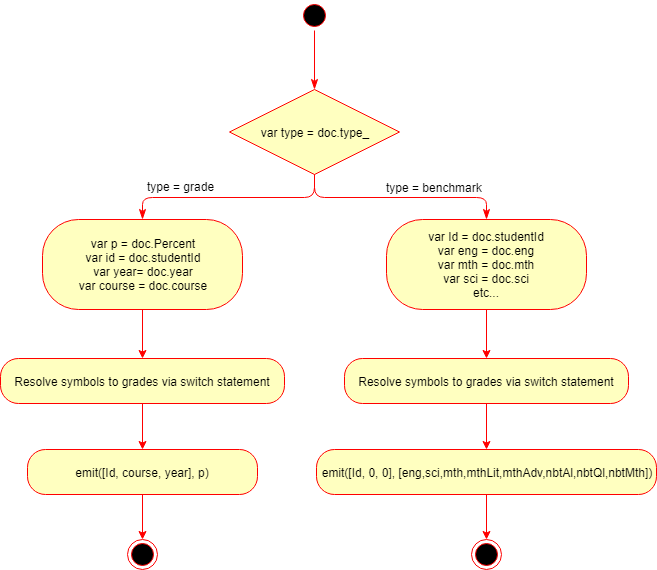
\includegraphics[scale=0.59]{./resources/figures/fig-mapfn-correlation-grades.png}
    \end{mdframed}
    \caption[\textit{Map}-function: \texorpdfstring{grades $\bowtie$ admissions}{Lg}]{\textbf{Figure \ref{fig-mapfn-correlation-grades}: \textit{Map}-function: \texorpdfstring{grades $\bowtie$ admissions}{Lg}}}
    \label{fig-mapfn-correlation-grades}
\end{figure}


\subsection{List Function: calculating correlation}
The list function is executed via a call to CouchDB's HTTP API. For the project the URI of that function call is \url{https://localhost:5984/msc/\_design/2-way-join/\_list/2-way-join-list/ 2-way-join-view?reduce=false}. On invocation the List function opens and scans the index iteratively processing each document (i.e. iteratively processing each student; first a student's demographic document is processed, then a student's grades documents are processed). The join is performed during list function execution alongside calculation of correlation coefficients according to the formula\footnote{\textit{x}: grade \%, \textit{y}: benchmark (\textit{r} is calculated for multiple \textit{y} values)}: \begin{spreadlines}{15pt}
    \begin{gather*}
        \intertext{\textit{Pearson Correlation Coefficient:}}
        r = \frac{N\sum{xy} - (\sum{x})(\sum{y})}{\sqrt{[N\sum{x^2} - (\sum{x})^2][N\sum{y^2} - (\sum{y})^2]}}
    \end{gather*}
\end{spreadlines}

When calculating variance (as shown previously), only a single data entity was used. As such the \_stats function could be used as a means of creating aggregations for corresponding values such as \textit{sum of squares}, \textit{sum} and \textit{count}, and then variance could be worked out in reference to these aggregated values. Working out correlation cannot make use of CouchDB's \_stats reduce function, since entities are reduced separately and only final aggregations of each entity are made available on data retrieval. For example, in reference to working out the numerator in reference to correlation: \begin{spreadlines}{15pt}
    \begin{gather*}
        N\sum{xy} - (\sum{x})(\sum{y})
    \end{gather*}
\end{spreadlines}

Using CouchDB's \_stats function only the $\sum{x}$ and $\sum{y}$ values are accessible when joining the two entities during list function execution, and not $x$ and $y$ values (similarly, the denominator of the formula could also not be calculated from \_stats function output). As such, to work out the correlation between grades and benchmarks requires aggregations across entities during list function execution; essentially the list function is used to aggregate numerical data from disparate entities by means of joins performed iteratively per student number. To achieve this, the list function is required to work with running totals as the index (the output of the map function without using a reduce function) is iterated over.

Output of the list function is configured to be a standard HTML page views within a browser, and accessed via the CouchDB endpoint: \url{http://localhost:5984/analysis-1/_design/analysis-1/_list/analysis-1/analysis-1.html}; the correlation between different benchmarking methods and grades is shown in Table \ref{tbl-correlation-grades}.

\begin{table}[H]
    \begin{threeparttable}
        \textbf{Table \ref{tbl-correlation-grades}}\par\medskip\par\medskip
        \caption{Correlation between different benchmarking methods and CSC1015F grades}
        \label{tbl-correlation-grades}
        \begin{tabularx}{\textwidth}{>{\hsize=1.3\hsize}X>{\hsize=0.7\hsize}Y}
            \toprule
            \mC{c}{Benchmark}                     & \mC{c}{$r$} \\
            \midrule
            Gr12 Eng \%                           & 0.287       \\
            Gr12 Sci \%                           & 0.465       \\
            Gr12 Mth \%                           & 0.447       \\
            NBT AL \%                             & 0.368       \\
            NBT QL \%                             & 0.533       \\
            NBT Mth \%                            & 0.510       \\
            Avg Gr12 \%                           & 0.485       \\
            Avg Gr12 \% (Dbl Mth)                 & 0.487       \\
            Avg Gr12 \% (Dbl Mth \& Sci)          & 0.493       \\
            Avg NBT \%                            & 0.583       \\
            Avg NBT \% (Dbl AL)                   & 0.559       \\
            Avg NBT \% (Dbl QL)                   & 0.580       \\
            Avg NBT \% (Dbl Mth)                  & 0.583       \\
            Avg NBT \% (Dbl AL/QL)                & 0.567       \\
            Avg NBT \% (Dbl AL/Mth)               & 0.570       \\
            Avg NBT \% (Dbl QL/Mth)               & 0.589       \\
            Avg Gr12 \& NBT                       & 0.610       \\
            Avg Gr12 \& NBT (Dbl Gr12 Mth)        & 0.587       \\
            Avg Gr12 \& NBT (Dbl Gr12 Mth \& Sci) & 0.578       \\
            \bottomrule
        \end{tabularx}
    \end{threeparttable}
\end{table}

Figure \ref{fig-listfn-correlation-grades}  TODO

\begin{figure}[H]
    \centering
    \begin{mdframed}
        \centering
        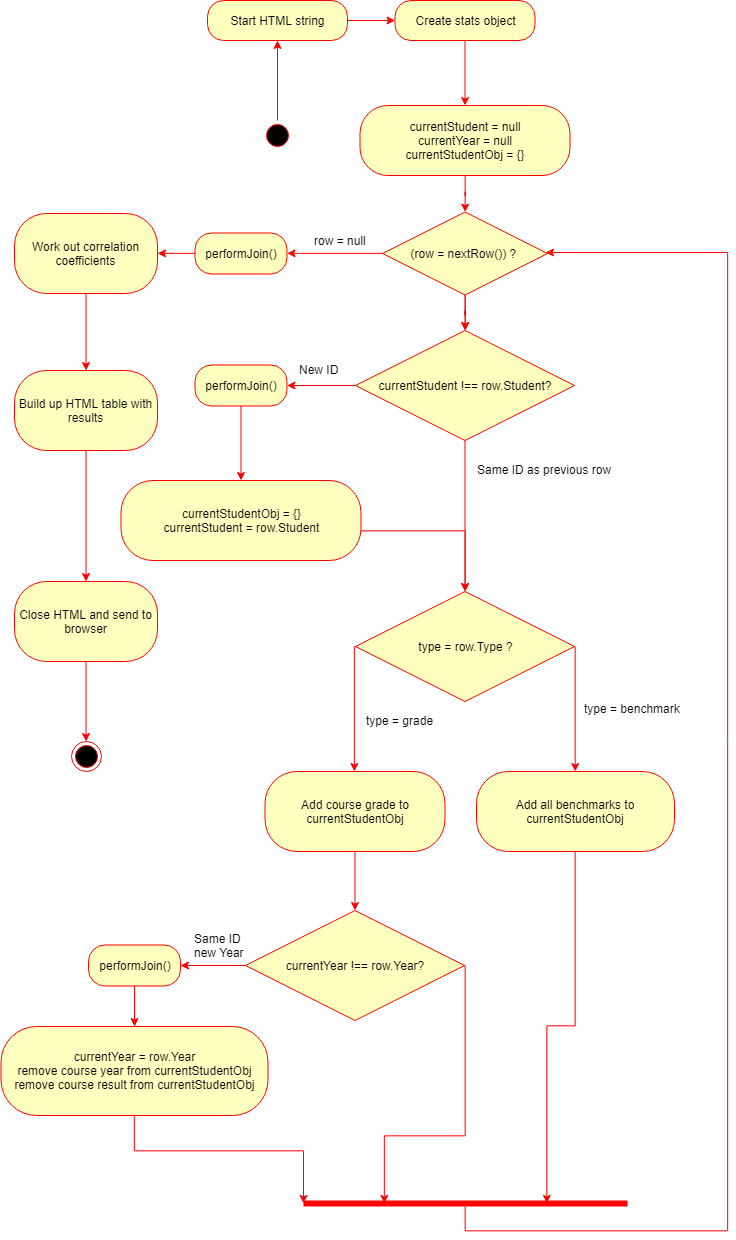
\includegraphics[scale=0.5]{./resources/figures/fig-listfn-correlation-grades.png}
    \end{mdframed}
    \caption[Grade/Benchmark correlation list function]{\textbf{Figure \ref{fig-listfn-correlation-grades}: Join/stats logic for grade/benchmark correlation analysis}}
    \label{fig-listfn-correlation-grades}
\end{figure}
